\documentclass[11pt, compress]{beamer}

\usetheme{m}

\usepackage{booktabs}
\usepackage[scale=2]{ccicons}
\usepackage{minted}
\usepackage{graphicx}
\usepackage{listings}

\usemintedstyle{trac}

\title{An entropically-secure covert channel in distributed version control systems}
\subtitle{}
\date{\today}
\author{Paul Chaignon, Damien Cr\'emilleux, Daryl Johnson}
\institute{Rochester Institute of Technology}

\begin{document}

%----------------------------------------------------------------------------------------
%	TITLE PAGE
%----------------------------------------------------------------------------------------
\begin{frame}
\titlepage 
\end{frame}


%----------------------------------------------------------------------------------------
%	Overview
%----------------------------------------------------------------------------------------
\begin{frame}
\frametitle{Overview} % Table of contents slide, comment this block out to remove it
\tableofcontents % Throughout your presentation, if you choose to use \section{} and \subsection{} commands, these will automatically be printed on this slide as an overview of your presentation
\end{frame}


%----------------------------------------------------------------------------------------
%	PRESENTATION SLIDES
%----------------------------------------------------------------------------------------
\section{Introduction}

\begin{frame}{Covert channels}
\vfill
Introduced by Lampson in 1973
\vfill
\begin{block}{Definition}
Any communication channel that can be exploited by a process to transfer information in a manner that violates the system's security policy.
\end{block}
\vfill
\end{frame}

\begin{frame}{Covert channels}
\begin{figure}
  \centering
    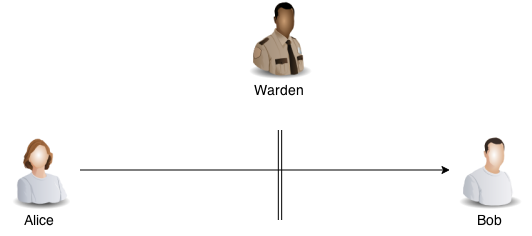
\includegraphics[width=0.8\textwidth]{images/covert_channel_1.png}
  %\caption{}
  \label{fig:covert_channel_1}
\end{figure}
\end{frame}

\begin{frame}{Covert channels}
\begin{figure}
  \centering
    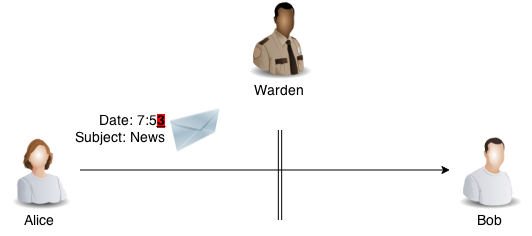
\includegraphics[width=0.8\textwidth]{images/covert_channel_2.png}
  %\caption{}
  \label{fig:covert_channel_2}
\end{figure}
\end{frame}


\section{Distributed version control systems}

\begin{frame}{Distributed version control systems}

\begin{itemize}
\item Used by developers to collaborate on software projects
\medskip
\item Managements of changes to documents or computer programs
\medskip
\item Widely used in companies
\medskip
\item Some distributed version control systems: \textbf{Git}, Bazaar, Mercurial, GNU arch
\end{itemize}

\end{frame}

\begin{frame}{Vocabulary}
\vfill
\begin{block}{Repository}
Set of files needed to manage a project (source code, changes, permissions, etc).
\end{block}
\vfill
\begin{block}{Commit}
A patch that can be applied to the repository, in order to obtain the modification sent by the developers.
\end{block}
\vfill
\end{frame}

\begin{frame}[fragile]{Commit}
\vfill
  \begin{lstlisting}[frame=single, breaklines=true, basicstyle=\small]
commit 231
tree cc7e48bd538188f75551fac0972840a7f6c2401f
parent 31463d4a762389f9b3d8fe872971e27c14dec645
author Xavier De Latourette <xd@gmail.com> 1412964284 -0400
committer Xavier De Latourette <xd@gmail.com> 1412964284 -0400
commit Modification of the README
  \end{lstlisting}
  \vfill
  All these information are used to obtain the hash (SHA-1) of the commit (e.g. d6cd1e2bd19e03a81132a23b2025920577f84e37).
The hash is needed because the system is distributed.
\end{frame}


\section{The covert channel}

\begin{frame}{Description}
\vfill
\begin{block}{Main idea}
Hide hexadecimal-encoded data in the SHA-1 hashes with partial hash collision.
\end{block}
\vfill
 d6cd1e2bd19e03a81132a23b2025920577f84e37 will become d6cd1e2bd19e03a81132a23b2025920577f84e\textbf{cc}
 \vfill

\end{frame}


\begin{frame}{Description}
\begin{itemize}
\item Any field of the commit can be changed to modify the hash
\item []
\item Addition of white spaces and tabulations to the end of the description text
\item []
\item Number of different descriptions that can be generated with a number of spaces and tabulations to p. 
\begin{equation*}
\label{eq:number_spaces}
N_p = \sum_{i=0}^{p} 2^i = 2^{p+1} - 1
\end{equation*}
\end{itemize}
\end{frame}



\begin{frame}{Analysis}

Covert channels can be defined by a set of properties:
\begin{itemize}
\item \textbf{Type}: storage, timing or behavioral covert channel.
The data is stored into hashes, it is a \textbf{storage} covert channel
\end{itemize}
\end{frame}

\begin{frame}{Analysis}
\begin{itemize}
\item \textbf{Robustness}: ability to survive any modification that may happen during the transmission. Distributed version control system rely on HTTP and hashes cannot be modified, so \textbf{highly robust}.
\end{itemize}
\end{frame}

\begin{frame}{Analysis}
\begin{itemize}
\item \textbf{Prevention}: the ease with which the channel can be disrupted. Commits need to have the same hash on all system, so it is \textbf{infeasible}.
\end{itemize}
\end{frame}

\begin{frame}{Analysis}
\begin{itemize}
\item \textbf{Detection}: the difficulty to detect the channel. Any text steganographic methods can be employed, this is \textbf{challenging}.
\end{itemize}
\end{frame}

\begin{frame}{Analysis}
\begin{itemize}
\item \textbf{Throughput}: the amount of data that can be transmitted in a given period of time.
The throughput depends of the number of characters ($k$) hidden in a hash. The number of attempts to obtain the right hash, for a probability $p$, is given by:
\begin{equation*}
\label{eq:num_attempts}
n > \frac{\log(1 - p)}{\log(1 - \frac{1}{2^{4k}})}
\end{equation*}

\end{itemize}

\end{frame}

\begin{frame}{Analysis}
\begin{figure}
    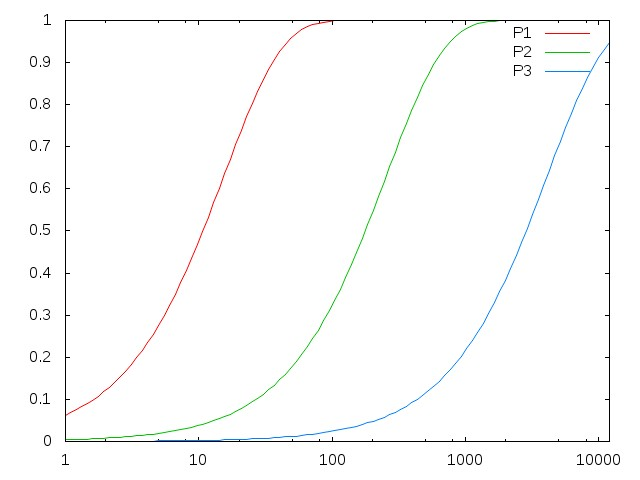
\includegraphics[width=0.8\textwidth]{images/plot.jpg}
    \caption{Probability of a partial collision as a function of the number attempts}
    \label{fig:plot}
\end{figure}
\end{frame}






\section{Experiments}

\begin{frame}{Disclaimer}
\vfill
All experiments have been carried on a standard laptop.
\vfill
\end{frame}

\begin{frame}{Hash collision}
\vfill
\begin{center}
    \begin{tabular}{ | c | c | c | c |}
    \hline
    Characters for the collision & 1  & 2 & 3 \\ \hline
    Time spent (ms) & 26 & 32 & 64  \\ \hline
    \end{tabular}
\end{center}
\vfill
\end{frame}

\begin{frame}{Transmission of a real message}
\vfill
\begin{center}
    \begin{tabular}{ | c | c | c | c | }
    \hline
    Length of the message (bytes) & 10  & 100  & 1000  \\ \hline
    Time spent (s) &  0.92  & 4.05  & 15  \\ \hline
    \end{tabular}
\end{center}
\vfill
This covert channel can be defined as a \textbf{high-bandwidth} covert channel.
\vfill
\end{frame}

\section{Detection through entropy measurements}

\begin{frame}{Entropy}
    \vfill
    \begin{block}{Formula}
        Information entropy defined by Shannon as:\\
        \begin{equation}
        H = - \sum_{i} p_i \log_2{p_i}
        \end{equation}
        $p_i$ the probability that the $i^{th}$ character appears in the data
    \end{block}
    \vfill
    \begin{block}{Examples}
        $H("aaaaaaaaaaaaaaaaaaaa") = 0$\\
        $H("b76ac7bab008ed7fdc2a1") = 3.42733$\\
        $H(\sum_i^{\infty} hash_i) \rightarrow 4$
    \end{block}
    \vfill
\end{frame}


\begin{frame}{Entropy measurements}
    \vfill
    \begin{block}{Worst case scenario}
        We want to send only Bs (66 in ASCII)\\
        The entropy will decrease because of the high number of 6\\
        -0.3 with a hundred hashes
    \end{block}
    \vfill
    \begin{block}{Real world scenario}
        We want to send a text\\
        Most values will be between 97 and 7A\\
        Decrease in entropy still noticeable
    \end{block}
    \vfill
\end{frame}


\begin{frame}{Solution 1}
    \vfill
    \begin{block}{Encryption}
        Let's Encrypt!\\
        Encrypted text will appear more random
    \end{block}
    \vfill
    \begin{block}{But...}
        We don't want any padding\\
        A lot of trouble for nothing
    \end{block}
    \vfill
\end{frame}


\begin{frame}{Solution 2}
    \vfill
    \begin{block}{XOR with a random number}
        PRNG with a shared seed\\
        Receiver and sender have the same random numbers\\
        Text XORed with the random numbers
    \end{block}
    \vfill
    \begin{block}{But...}
        Today's PRNGs have many properties\\
        We only need it to appear random
    \end{block}
    \vfill
\end{frame}


\begin{frame}{Solution 3}
    \vfill
    \begin{block}{Linear Feedback Shift Register}
        Was used as a PRNG (back in the days)\\
        Very simple and fast
    \end{block}
    \vfill
\end{frame}


\begin{frame}{Solutions}
    \vfill
    \begin{block}{Solutions}
        \begin{itemize}
        \item Symmetric cipher
        \item XOR with PRNG output
        \item XOR with LFSR ouput
        \end{itemize}
    \end{block}
    \vfill
    \begin{block}{Experiments}
        All solutions were able to keep the entropy constant
    \end{block}
    \vfill
\end{frame}




\section{Conclusion}
\begin{frame}{Conclusion}
\begin{itemize}
\item Innovative covert channel
\item []
\item Entropically-secure channel
\item []
\item Experiments prove its effectiveness
\end{itemize}
\end{frame}


\plain{}{Questions or comments?}

\end{document}
